% The generic preamble
\documentclass[10pt,letterpaper,fleqn,titlepage]{report}

% Define packages to use
\usepackage{natbib}
\usepackage[dvips]{graphicx,color}
\usepackage{amsmath,amssymb}
\usepackage{bm}
\usepackage{caption}
\usepackage{xr}
\usepackage{ifthen}
\usepackage[dvipdfm,colorlinks,linkcolor=blue,citecolor=blue,urlcolor=blue]{hyperref}
\usepackage{fancybox}
\usepackage{textcomp}
\usepackage{fancyhdr}
\usepackage{titlesec}
\usepackage{multirow}
\usepackage{alltt}
\usepackage{svn}
\usepackage{longtable}

\titleformat{\chapter}[frame]
  {\normalfont}
  {\filright\slshape\Huge\enspace\thechapter\enspace}
  {8pt}
  {\normalfont\Huge\filcenter\slshape\sffamily} 

\titleformat{\section}[hang]
  {\normalfont}
  {\filright\sffamily\bfseries\Large\thesection}
  {5pt}
  {\normalfont\Large\filright\sffamily\bfseries}[\vspace{2pt}\titlerule]

\titleformat{\subsection}[hang]
  {\normalfont}
  {\filright\slshape\sffamily\large\thesubsection}
  {5pt}
  {\normalfont\large\filright\slshape\sffamily} 
  
% Redefine default page
\setlength{\textheight}{9.0in}  % 1" above and below
\setlength{\textwidth}{6.75in}   % 0.5" left and right
\setlength{\oddsidemargin}{-0.25in}
\setlength{\topmargin}{0.0pt}
\setlength{\headsep}{16.0pt}

% Redefine default paragraph
\setlength{\parindent}{0pt}
\setlength{\parskip}{1.5ex plus 0.5ex minus 0.2ex}

% Define caption width and default fonts
\setlength{\captionmargin}{0.5in}
\renewcommand{\captionfont}{\sffamily}
\renewcommand{\captionlabelfont}{\bfseries\sffamily}

% Defined commands
\newcommand{\superscript}[1]{\ensuremath{^\textrm{#1}}}
\newcommand{\subscript}[1]{\ensuremath{_\textrm{#1}}}
\newcommand{\invcm}{\textrm{cm\superscript{-1}}}
\newcommand{\micron}{\ensuremath{\mu\textrm{m}}}
\newcommand{\textbfm}[1]{\boldmath\ensuremath{#1}\unboldmath}
\newcommand{\water}{\textrm{H\subscript{2}O}}
\newcommand{\carbondioxide}{\textrm{CO\subscript{2}}}
\newcommand{\ozone}{\textrm{O\subscript{3}}}
\newcommand{\methane}{\textrm{CH\subscript{4}}}
\newcommand{\nitrousoxide}{\textrm{N\subscript{2}O}}
\newcommand{\carbonmonoxide}{\textrm{CO}}

% Define how equations are numbered
\numberwithin{equation}{chapter}
\numberwithin{figure}{chapter}
\numberwithin{table}{chapter}

% Space/nudging commands
\newcommand{\rb}[1]{\raisebox{1.5ex}[0pt]{#1}}

%Redefine the enumerate environment to decrease the item spacing.
\let\oldenumerate=\enumerate
\let\endoldenumerate=\endenumerate
\renewenvironment{enumerate}{%
  \begin{oldenumerate}%
    \setlength{\itemsep}{0ex}%
  }%
  {%
  \end{oldenumerate}%
  }

% Define a command for title page author email footnote
\newcommand{\email}[1]
{%
  \renewcommand{\thefootnote}{\alph{footnote}}%
  \footnote{#1}
  \renewcommand{\thefootnote}{\arabic{footnote}}
}

% Redefine the maketitle macro
\makeatletter
\renewcommand{\maketitle}
{%
  \thispagestyle{empty}
  \vspace*{1in}
  \begin{center}%
     \sffamily
     {\huge\bfseries Joint Center for Satellite Data Assimilation\par}%
  \end{center}
  \begin{flushleft}%
     \sffamily
     \vspace*{0.5in}
     {\Large\bfseries CRTM: \@title\par}%
     \medskip
     {\large\@author\par}%
     \medskip
     {\large\@date\par}%
     \bigskip\hrule\vspace*{2pc}%
  \end{flushleft}%
  \newpage
  \setcounter{footnote}{0}
}
\makeatother


% Define a command for a DRAFT watermark
\usepackage{eso-pic}
\newcommand{\draftwatermark}
{
  \AddToShipoutPicture{%
    \definecolor{lightgray}{gray}{.85}
    \setlength{\unitlength}{1in}
    \put(2.5,3.5){%
      \rotatebox{45}{%
        \resizebox{4in}{1in}{%
          \textsf{\textcolor{lightgray}{DRAFT}}
        }
      }
    }
  }
}


% Include files
\includeonly{SRF_Data_Plots.app,Tfit_Data_Plots.app}

% Subversion keywords
\SVN $Date$
\SVN $Revision$

% Title info
\title{INSAT-3D Imager and Sounder Spectral Response Function Processing}
\author{Paul van Delst\email{paul.vandelst@noaa.gov}\\NCEP/EMC/IMSG}
\date{\SVNDate ; rev\SVNRevision}
\docnumber{3}
\docseries{CRTM}


%-------------------------------------------------------------------------------
%                            Ze document begins...
%-------------------------------------------------------------------------------
\begin{document}
\maketitle

\draftwatermark

% The front matter
%=================
\thispagestyle{empty}
\vspace*{10cm}
\begin{center}
  {\sffamily\Large\bfseries Change History}
  \begin{table}[htp]
    \centering
    \begin{tabular}{|p{2cm}|p{3cm}|p{8cm}|}
      \hline
      \sffamily\textbf{Date} & \sffamily\textbf{Author} & \sffamily\textbf{Change}\\
      \hline\hline
      2013-11-21 & Paul van Delst & Initial draft.\\
      \hline
    \end{tabular}
  \end{table}
\end{center}
\clearpage
\pagestyle{fancy}
\fancyhead[LE,RO]{\sffamily \rightmark}
\fancyhead[LO,RE]{\sffamily \leftmark}
\pagenumbering{arabic}
\setcounter{page}{1}


% The main matter
%================

\section{Introduction}
%=====================
This document describes the pre-processing applied to the INSAT-3D Imager and Sounder instruments spectral response functions (SRFs), obtained from \cite{INSAT3D_SRF_Data}, to prepare for use in the CRTM processing chain. The SRFs are used to generate channel central frequencies, as well as in the convolution of monochromatic quantities such as Planck radiances or line-by-line (LBL) model generated transmittances to produce such things as polychromatic correction coefficients and instrument resolution transmittances. The latter, for a diverse set of atmospheric profiles, are then regressed against a set of predictors to produce the fast transmittance model coefficients used by the CRTM.


\subsection{Computation of the channel central frequency}
%--------------------------------------------------------
The computed imager and sounder channel central frequencies, $\nu_0$, are the first moments of the defined SRF, $\phi(\nu)$,
\begin{equation}
  \nu_0 = \frac{\displaystyle\int{\nu\:\phi(\nu)\ud \nu}}{\displaystyle\int{\phi(\nu)\ud \nu}}
\end{equation}


\subsection{Computation of polychromatic correction coefficients}
%----------------------------------------------------------------
In the CRTM, the conversion of \emph{channel resolution} radiances to brightness temperatures has to take the channel bandwidth into account. For any channel, the regression relation to be solved is

\begin{equation}
  a_0 + a_1T + \ldots = \frac{\displaystyle k_1}{\displaystyle \ln\left[\frac{k_2}{R(T)}+1\right]} = Y(T)
\end{equation}
where
\begin{equation}
  \begin{array}{r@{\;=\;}l}
         T &\mbox{brightness temperature} \\
        a_j&\mbox{regression coefficients} \\
    k_1,k_2&\mbox{Planck coefficients} \\
       R(T)&\mbox{channel radiance} \\
       Y(T)&\mbox{``effective'' brightness temperature}
  \end{array}
\end{equation}
and the channel radiances used to determine the effective temperatures, $Y(T)$, are computed the usual way
\begin{equation}
  R(T) = \frac{\displaystyle\int{B(T,\nu)\:\phi(\nu)\ud \nu}}{\displaystyle\int{\phi(\nu)\ud \nu}}
\end{equation}
The quantity minimised to obtain the $a_j$ coefficients is
\begin{equation}
  \left[ \sum_{j=0}^{M}a_j T_{i} - Y(T_{i}) \right]^2 \quad\mbox{for}\quad T_i = 150K, \ldots, 340K \;\mbox{ in 5K steps.}
\end{equation}
Currently the number of coefficients is fixed at two (i.e. $M=1$).



\newpage
\section{Summary}
%================

The following tables list the computed central frequencies and polychromatic correction coefficients for the imager and sounder instruments. Plots of the SRF data are shown in appendix \ref{app.srf_data_plots}. The temperature fit residuals each channel are shown in appendix \ref{app.tfit_data_plots}.

\subsection{Imager}
%------------------

\begin{table}[htp]
  \centering
  \begin{tabular}{c *{3}{c r@{.}l}}
    \hline
    \sffamily{Imager} & & \multicolumn{2}{c}{$f_0$} & & \multicolumn{2}{c}{$a_0$ \textsf{(offset)}} & & \multicolumn{2}{c}{$a_1$ \textsf{(slope)}} \\
    \sffamily{Channel} & & \multicolumn{2}{c}{\sffamily{(cm\superscript{-1})}} & & \multicolumn{2}{c}{\sffamily{(K)}} & & \multicolumn{2}{c}{\sffamily{(K/K)}}  \\
    \hline\hline
    3  & & 2548&29790 & & 0&39296299 & & 0&99943449 \\
    4  & & 1454&64282 & & 0&62968299 & & 0&99850810 \\
    5  & &  924&84481 & & 0&38038615 & & 0&99868849 \\
    6  & &  836&86673 & & 0&26436608 & & 0&99900546 \\
    \hline
  \end{tabular}
  \caption{The computed INSAT-3D Imager channel central frequencies and polychromatic correction coefficients.}
  \label{tab:imgr_insat3d_results}
\end{table}


\subsection{Sounder}
%-------------------

\begin{table}[htp]
  \centering
  \begin{tabular}{c *{3}{c r@{.}l}}
    \hline
    \sffamily{Sounder} & & \multicolumn{2}{c}{$f_0$} & & \multicolumn{2}{c}{$a_0$ \textsf{(offset)}} & & \multicolumn{2}{c}{$a_1$ \textsf{(slope)}} \\
    \sffamily{Channel} & & \multicolumn{2}{c}{\sffamily{(cm\superscript{-1})}} & & \multicolumn{2}{c}{\sffamily{(K)}} & & \multicolumn{2}{c}{\sffamily{(K/K)}}  \\
    \hline\hline
    1 & &  681&64590 & & 0&03409436 & & 0&99984374 \\
    2 & &  698&53274 & & 0&03406585 & & 0&99984795 \\
    3 & &  712&09025 & & 0&02766887 & & 0&99987899 \\
    4 & &  733&02306 & & 0&04079706 & & 0&99982672 \\
    5 & &  750&71900 & & 0&04177552 & & 0&99982661 \\
    6 & &  792&59666 & & 0&09970706 & & 0&99960677 \\
    7 & &  834&24958 & & 0&20132505 & & 0&99924102 \\
    8 & &  906&05831 & & 0&17250629 & & 0&99939518 \\
    9 & & 1029&32245 & & 0&05587906 & & 0&99982373 \\
   10 & & 1344&46841 & & 0&23484069 & & 0&99940475 \\
   11 & & 1422&08644 & & 0&59108846 & & 0&99855512 \\
   12 & & 1530&54996 & & 0&34706350 & & 0&99920985 \\
   13 & & 2183&53822 & & 0&03188206 & & 0&99994688 \\
   14 & & 2209&08333 & & 0&03181492 & & 0&99994761 \\
   15 & & 2241&07074 & & 0&03815789 & & 0&99993782 \\
   16 & & 2419&76611 & & 0&06485661 & & 0&99990158 \\
   17 & & 2510&05083 & & 0&07352145 & & 0&99989162 \\
   18 & & 2657&62744 & & 0&26932455 & & 0&99962546 \\
    \hline
  \end{tabular}
  \caption{The computed INSAT-3D Sounder channel central frequencies and polychromatic correction coefficients.}
  \label{tab:sndr_insat3d_results}
\end{table}



\newpage
\section{Truncation of original data}
%====================================
\label{sec:data_truncation}

The original SRFs were reported on the same frequency grid for all channels in an instrument, with out-of-band responses set to zero. To minimise the number of frequencies for which LBL calculations would be done, the SRF data were truncated to eliminate the zero-valued out-of-band elements.

\subsection{Imager}
%------------------
The truncation frequencies for the imager instrument are shown in tables \ref{tab:imgr_insat3d_truncation}. The truncation points were selected by visual inspection.

\begin{table}[htp]
  \centering
  \begin{tabular}{c *{2}{c r@{.}l}}
    \hline
    \sffamily{Sounder} & & \multicolumn{2}{c}{$f_1$} & & \multicolumn{2}{c}{$f_2$}  \\
    \sffamily{Channel} & & \multicolumn{2}{c}{\sffamily{(cm\superscript{-1})}} & & \multicolumn{2}{c}{\sffamily{(cm\superscript{-1})}} \\
    \hline\hline
    3 & & 2450&00 & & 2650&00  \\
    4 & & 1350&00 & & 1600&00  \\
    5 & &  860&00 & &  990&00  \\
    6 & &  780&00 & &  890&00  \\
    \hline
  \end{tabular}
  \caption{The frequencies at which the original INSAT-3D Imager channel SRFs were truncated prior to processing.}
  \label{tab:imgr_insat3d_truncation}
\end{table}

The ``character'' of the imager SRFs at low response levels near the truncations points are shown in figure \ref{fig:imgr_ch3-6_trunc}

\begin{figure}[H]
  \centering
  \begin{tabular}{c c}
    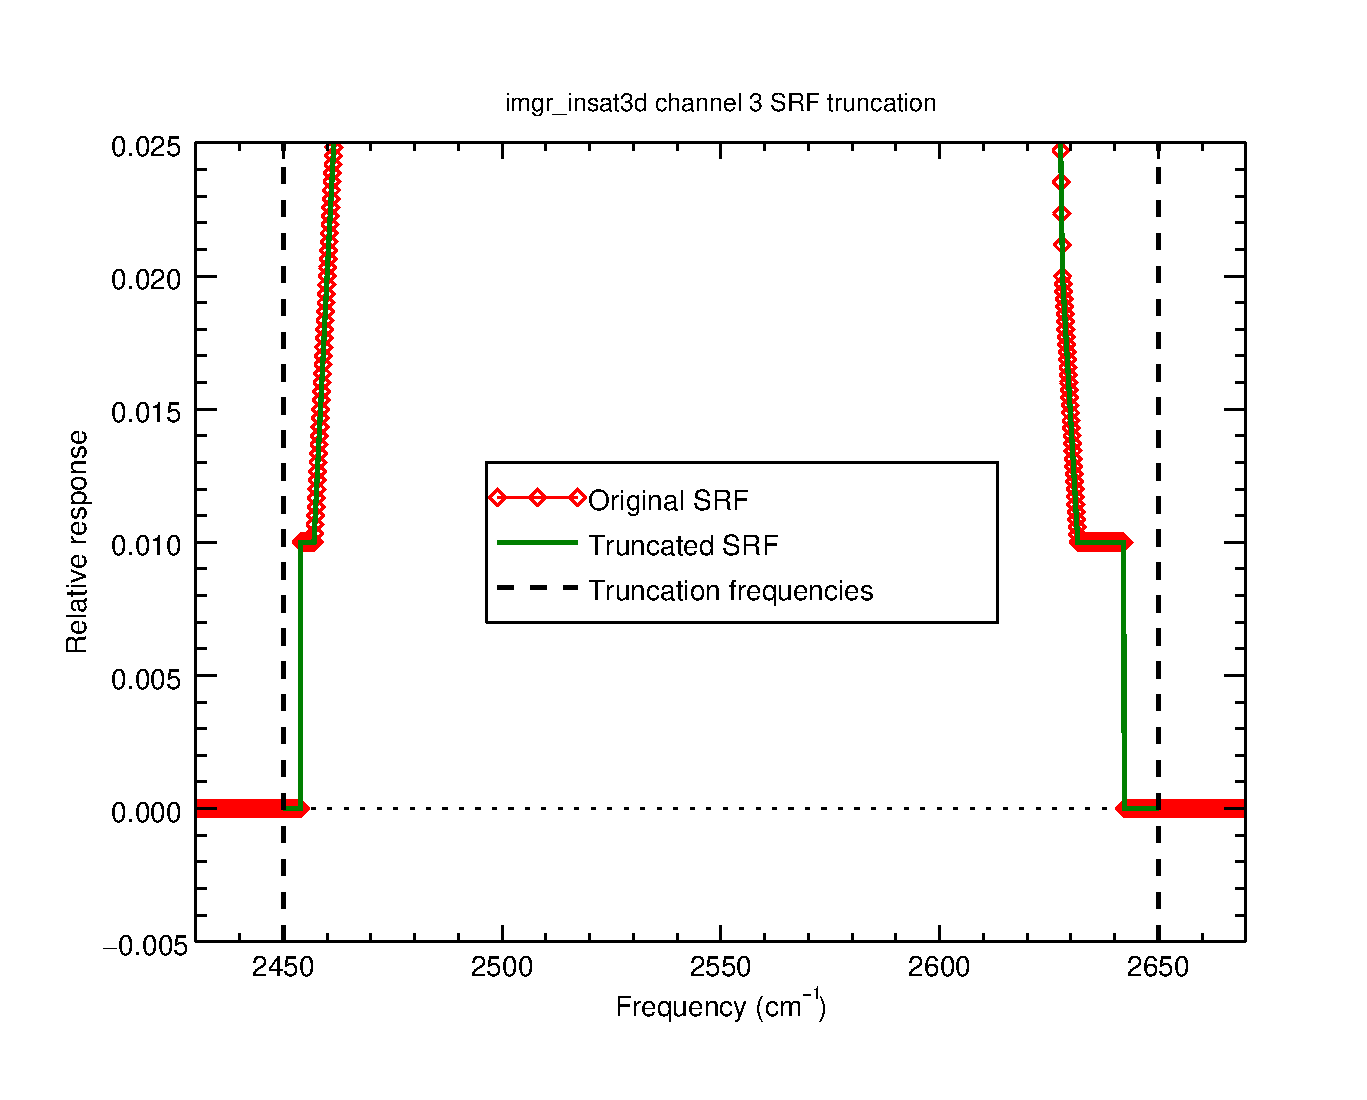
\includegraphics[scale=0.35]{graphics/imgr/trunc/imgr_insat3d-3.trunc.eps} &
    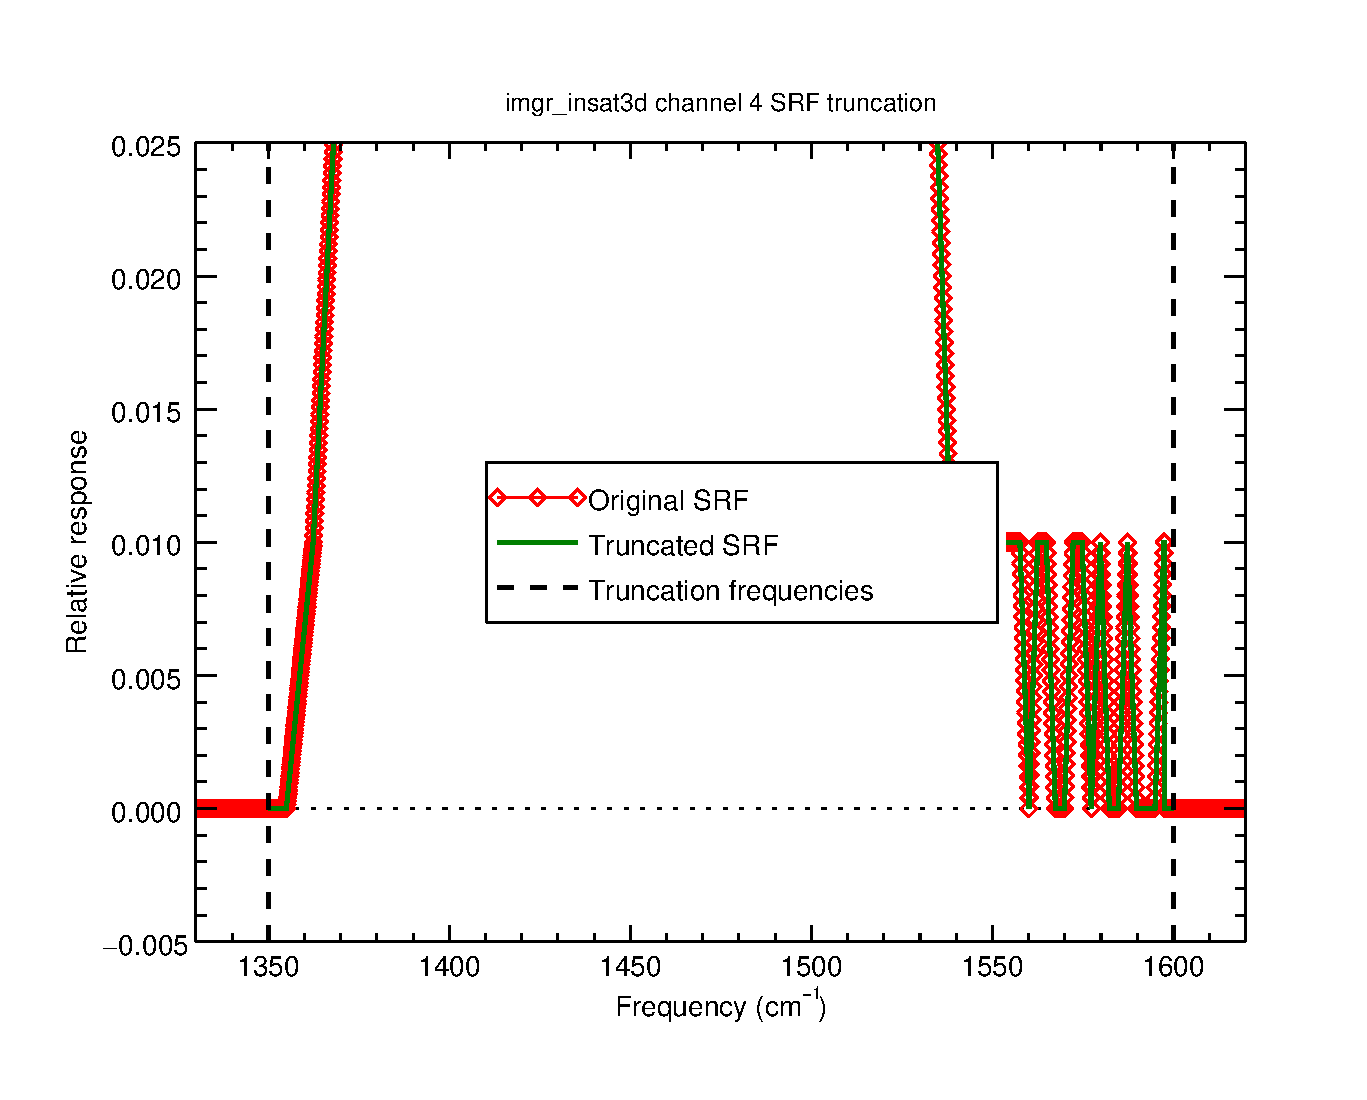
\includegraphics[scale=0.35]{graphics/imgr/trunc/imgr_insat3d-4.trunc.eps} \\
    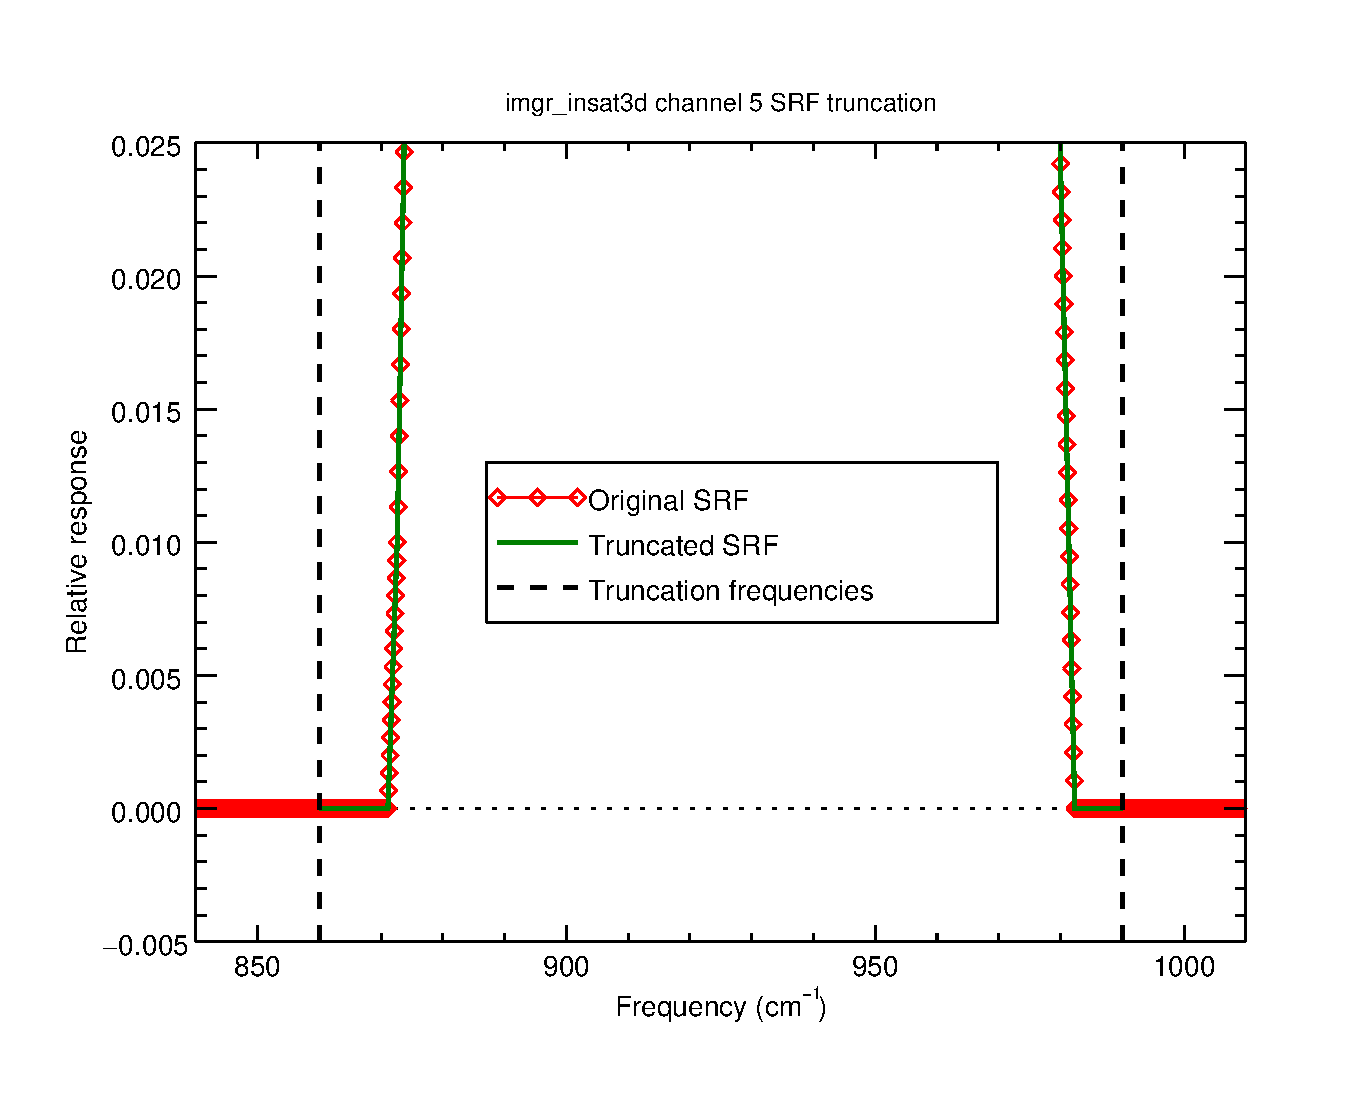
\includegraphics[scale=0.35]{graphics/imgr/trunc/imgr_insat3d-5.trunc.eps} &
    \includegraphics[scale=0.35]{graphics/imgr/trunc/imgr_insat3d-6.trunc.eps}
  \end{tabular}
  \caption{INSAT-3D Imager channels 3-6 SRFs at low response levels near the trunctiopn frequencies.}
  \label{fig:imgr_ch3-6_trunc}
\end{figure}


\subsection{Sounder}
%-------------------
The truncation frequencies for the sounder instrument are shown in table \ref{tab:sndr_insat3d_truncation}. The truncation points were selected automatically by determining the first non-zero point either side of the SRF, and then extending back 20 data points.

\begin{table}[htp]
  \centering
  \begin{tabular}{c *{2}{c r@{.}l}}
    \hline
    \sffamily{Sounder} & & \multicolumn{2}{c}{$f_1$} & & \multicolumn{2}{c}{$f_2$}  \\
    \sffamily{Channel} & & \multicolumn{2}{c}{\sffamily{(cm\superscript{-1})}} & & \multicolumn{2}{c}{\sffamily{(cm\superscript{-1})}} \\
    \hline\hline
     1 & &   656&20 & &  708&20 \\
     2 & &   671&70 & &  728&70 \\
     3 & &   687&20 & &  741&20 \\
     4 & &   702&10 & &  768&80 \\
     5 & &   715&20 & &  784&30 \\
     6 & &   739&30 & &  853&90 \\
     7 & &   753&70 & &  888&30 \\
     8 & &   856&90 & &  996&70 \\
     9 & &   993&60 & & 1069&90 \\
    10 & &  1253&30 & & 1427&60 \\
    11 & &  1259&80 & & 1543&80 \\
    12 & &  1427&60 & & 1630&00 \\
    13 & &  2151&00 & & 2217&20 \\
    14 & &  2179&10 & & 2245&10 \\
    15 & &  2207&60 & & 2279&80 \\
    16 & &  2379&60 & & 2462&50 \\
    17 & &  2458&70 & & 2557&50 \\
    18 & &  2580&10 & & 2741&60 \\
    \hline
  \end{tabular}
  \caption{The frequencies at which the original INSAT-3D Sounder channel SRFs were truncated prior to processing.}
  \label{tab:sndr_insat3d_truncation}
\end{table}

The ``character'' of a selection of the sounder SRFs at low response levels near the truncations points are shown in figure \ref{fig:sndr_selection_trunc}. 

\begin{figure}[H]
  \centering
  \begin{tabular}{c c}
    \includegraphics[scale=0.35]{graphics/sndr/trunc/sndr_insat3d-1.trunc.eps} &
    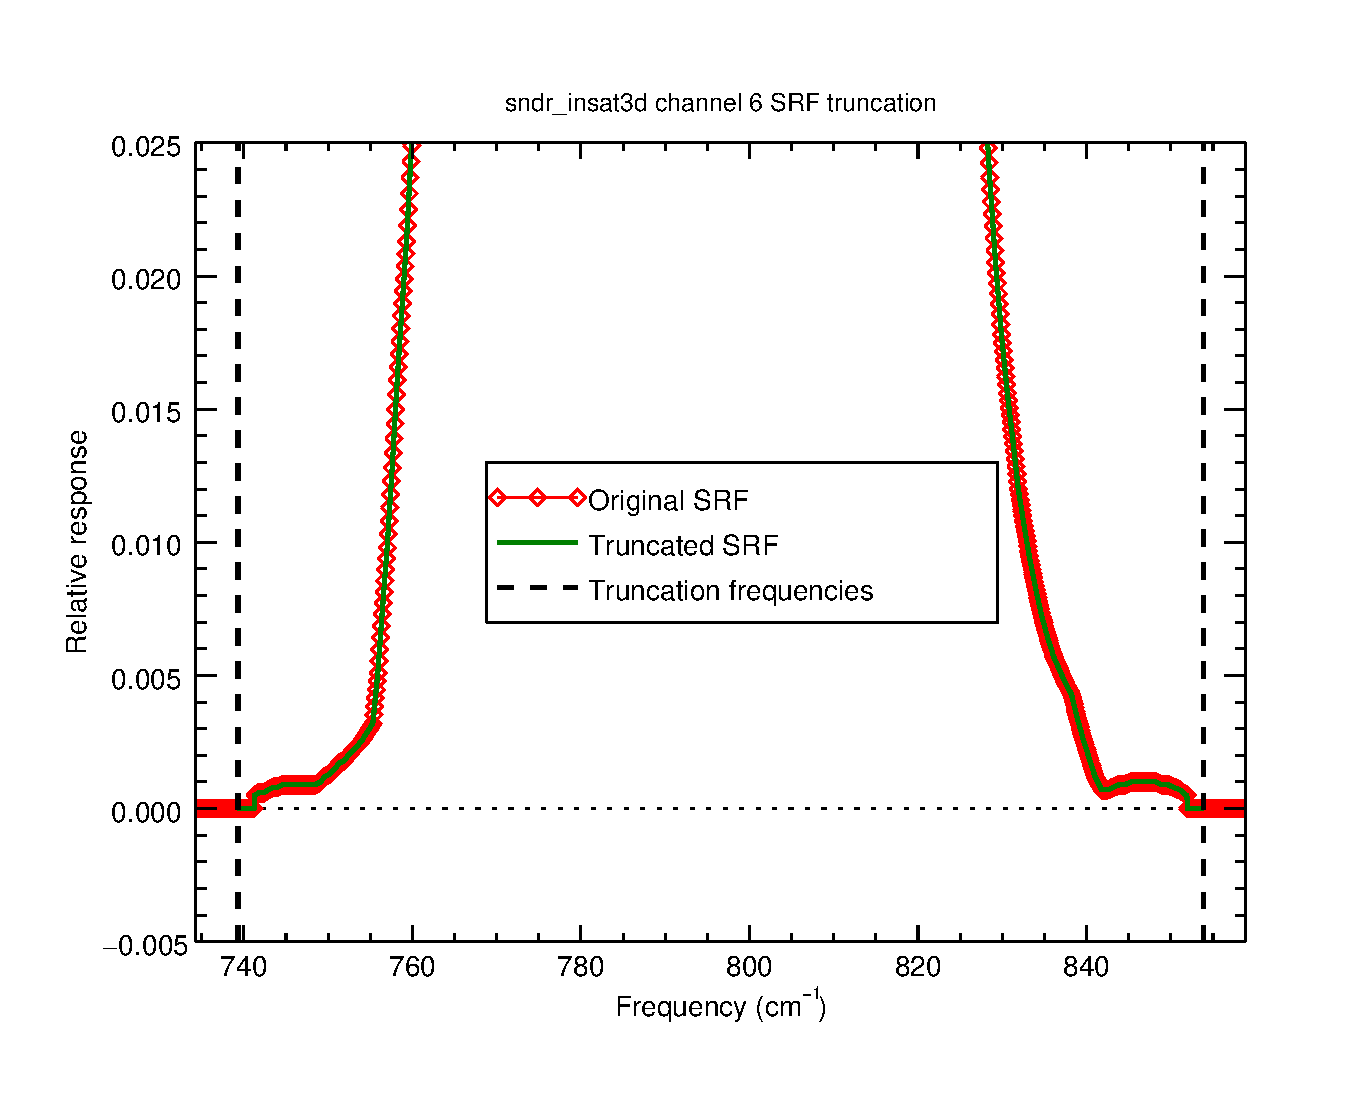
\includegraphics[scale=0.35]{graphics/sndr/trunc/sndr_insat3d-6.trunc.eps} \\
    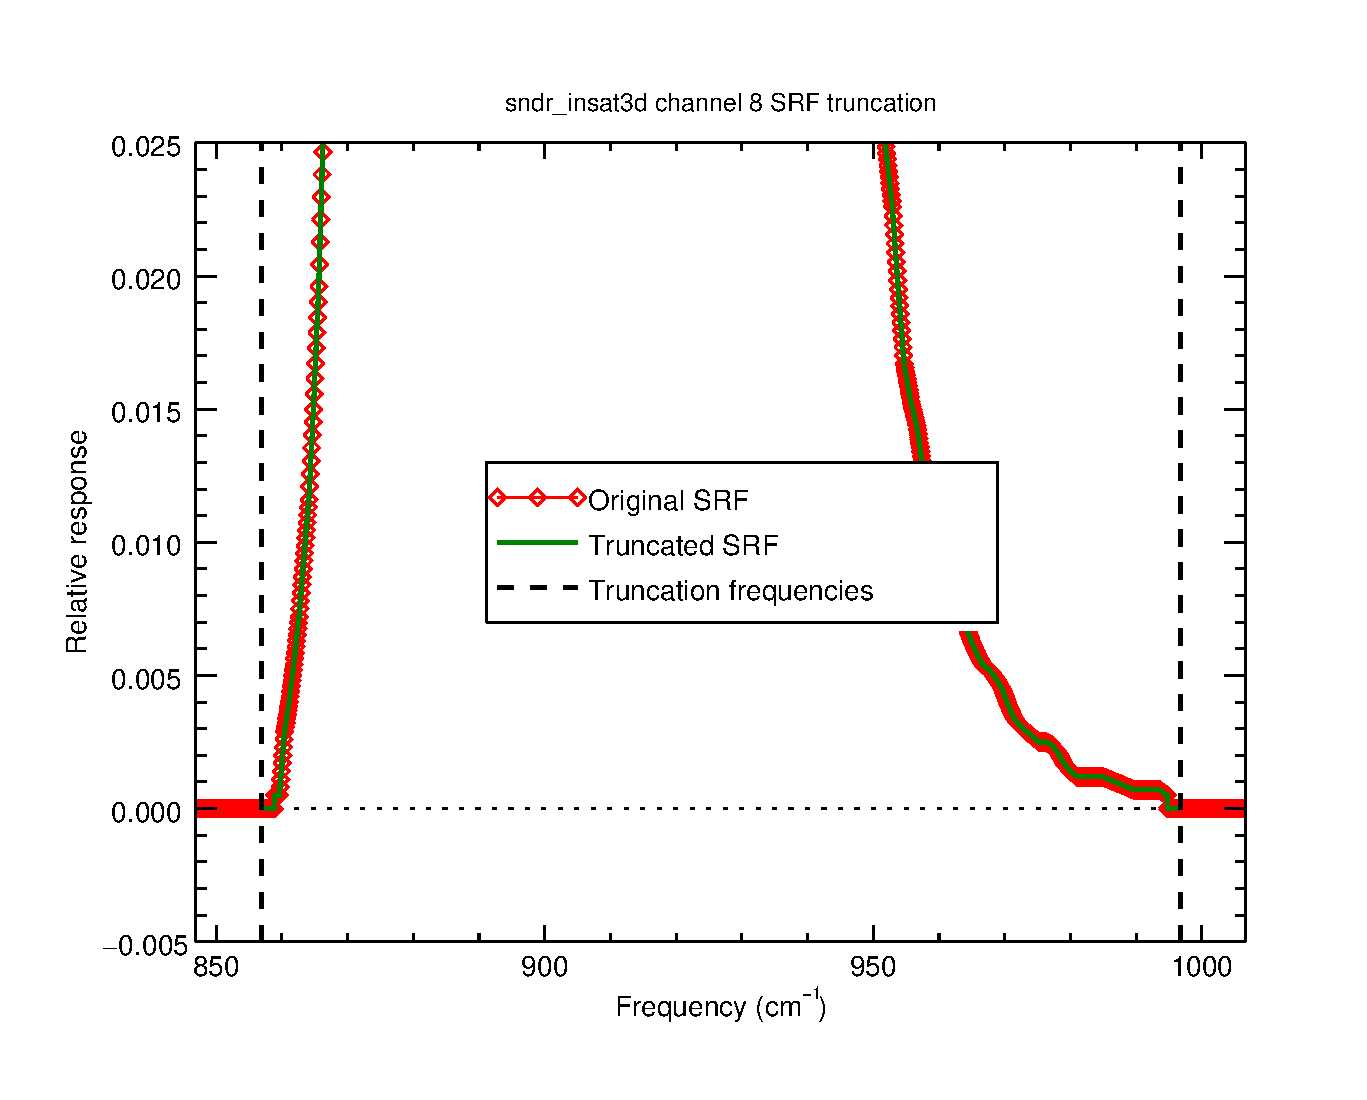
\includegraphics[scale=0.35]{graphics/sndr/trunc/sndr_insat3d-8.trunc.eps} &
    \includegraphics[scale=0.35]{graphics/sndr/trunc/sndr_insat3d-10.trunc.eps}
  \end{tabular}
  \caption{A selection of INSAT-3D Sounder channel SRFs at low response levels near the trunction frequencies.}
  \label{fig:sndr_selection_trunc}
\end{figure}


% The references section
%=======================
\clearpage
\bibliographystyle{plainnat}
\bibliography{bibliography}


% The appendices section
%=======================
\begin{appendix}
  \phantomsection
\section{GMI SRF Data Plots}
%===========================
\label{app.srf_data_plots}

\addcontentsline{toc}{subsection}{Channels 1-3}
\begin{figure}[H]
  \centering
  \begin{tabular}{c c}
    \multicolumn{2}{c}{\sffamily\textbf{Channel 1}}\\
    \includegraphics[scale=0.35]{graphics/lin/gmi_gpm-1.eps} &
    \includegraphics[scale=0.35]{graphics/log/gmi_gpm-1.eps} \\
    \multicolumn{2}{c}{\sffamily\textbf{Channel 2}}\\
    \includegraphics[scale=0.35]{graphics/lin/gmi_gpm-2.eps} &
    \includegraphics[scale=0.35]{graphics/log/gmi_gpm-2.eps} \\
    \multicolumn{2}{c}{\sffamily\textbf{Channel 3}}\\
    \includegraphics[scale=0.35]{graphics/lin/gmi_gpm-3.eps} &
    \includegraphics[scale=0.35]{graphics/log/gmi_gpm-3.eps}
  \end{tabular}
  \caption{GMI channels 1-3 responses for the three test temperatures: $T_{NOM}$ (25\textdegree{}C), $T_{LO}$ (-10\textdegree{}C), and $T_{HI}$ (45\textdegree{}C). Vertical dashed lines are the locations of the computed central frequencies. \textbf{(Left)} Linear y-axis. \textbf{(Right)} Base-10 logarithmic y-axis.}
  \label{fig:ch1-3_response}
\end{figure}

\addcontentsline{toc}{subsection}{Channels 4-6}
\begin{figure}[H]
  \centering
  \begin{tabular}{c c}
    \multicolumn{2}{c}{\sffamily\textbf{Channel 4}}\\
    \includegraphics[scale=0.35]{graphics/lin/gmi_gpm-4.eps} &
    \includegraphics[scale=0.35]{graphics/log/gmi_gpm-4.eps} \\
    \multicolumn{2}{c}{\sffamily\textbf{Channel 5}}\\
    \includegraphics[scale=0.35]{graphics/lin/gmi_gpm-5.eps} &
    \includegraphics[scale=0.35]{graphics/log/gmi_gpm-5.eps} \\
    \multicolumn{2}{c}{\sffamily\textbf{Channel 6}}\\
    \includegraphics[scale=0.35]{graphics/lin/gmi_gpm-6.eps} &
    \includegraphics[scale=0.35]{graphics/log/gmi_gpm-6.eps}
  \end{tabular}
  \caption{GMI channels 4-6 responses for the three test temperatures: $T_{NOM}$ (25\textdegree{}C), $T_{LO}$ (-10\textdegree{}C), and $T_{HI}$ (45\textdegree{}C). Vertical dashed lines are the locations of the computed central frequencies. \textbf{(Left)} Linear y-axis. \textbf{(Right)} Base-10 logarithmic y-axis.}
  \label{fig:ch4-6_response}
\end{figure}

\addcontentsline{toc}{subsection}{Channels 7-9}
\begin{figure}[H]
  \centering
  \begin{tabular}{c c}
    \multicolumn{2}{c}{\sffamily\textbf{Channel 7}}\\
    \includegraphics[scale=0.35]{graphics/lin/gmi_gpm-7.eps} &
    \includegraphics[scale=0.35]{graphics/log/gmi_gpm-7.eps} \\
    \multicolumn{2}{c}{\sffamily\textbf{Channel 8}}\\
    \includegraphics[scale=0.35]{graphics/lin/gmi_gpm-8.eps} &
    \includegraphics[scale=0.35]{graphics/log/gmi_gpm-8.eps} \\
    \multicolumn{2}{c}{\sffamily\textbf{Channel 9}}\\
    \includegraphics[scale=0.35]{graphics/lin/gmi_gpm-9.eps} &
    \includegraphics[scale=0.35]{graphics/log/gmi_gpm-9.eps}
  \end{tabular}
  \caption{GMI channels 7-9 responses for the three test temperatures: $T_{NOM}$ (25\textdegree{}C), $T_{LO}$ (-10\textdegree{}C), and $T_{HI}$ (45\textdegree{}C). Vertical dashed lines are the locations of the computed central frequencies. \textbf{(Left)} Linear y-axis. \textbf{(Right)} Base-10 logarithmic y-axis.}
  \label{fig:ch7-9_response}
\end{figure}

\addcontentsline{toc}{subsection}{Channels 10-12}
\begin{figure}[H]
  \centering
  \begin{tabular}{c c}
    \multicolumn{2}{c}{\sffamily\textbf{Channel 10}}\\
    \includegraphics[scale=0.35]{graphics/lin/gmi_gpm-10.eps} &
    \includegraphics[scale=0.35]{graphics/log/gmi_gpm-10.eps} \\
    \multicolumn{2}{c}{\sffamily\textbf{Channel 11}}\\
    \includegraphics[scale=0.35]{graphics/lin/gmi_gpm-11.eps} &
    \includegraphics[scale=0.35]{graphics/log/gmi_gpm-11.eps} \\
    \multicolumn{2}{c}{\sffamily\textbf{Channel 12}}\\
    \includegraphics[scale=0.35]{graphics/lin/gmi_gpm-12.eps} &
    \includegraphics[scale=0.35]{graphics/log/gmi_gpm-12.eps}
  \end{tabular}
  \caption{GMI channels 10-12 responses for the three test temperatures: $T_{NOM}$ (25\textdegree{}C), $T_{LO}$ (-10\textdegree{}C), and $T_{HI}$ (45\textdegree{}C). \textbf{(Left)} Linear y-axis. \textbf{(Right)} Base-10 logarithmic y-axis.}
  \label{fig:ch10-12_response}
\end{figure}

\addcontentsline{toc}{subsection}{Channel 13}
\begin{figure}[H]
  \centering
  \begin{tabular}{c c}
    \multicolumn{2}{c}{\sffamily\textbf{Channel 13}}\\
    \includegraphics[scale=0.35]{graphics/lin/gmi_gpm-13.eps} &
    \includegraphics[scale=0.35]{graphics/log/gmi_gpm-13.eps}
  \end{tabular}
  \caption{GMI channel 13 responses for the three test temperatures: $T_{NOM}$ (25\textdegree{}C), $T_{LO}$ (-10\textdegree{}C), and $T_{HI}$ (45\textdegree{}C). \textbf{(Left)} Linear y-axis. \textbf{(Right)} Base-10 logarithmic y-axis.}
  \label{fig:ch10-13_response}
\end{figure}

  \section{Polychromatic Correction Temperature Fit Residual Data Plots}
%=====================================================================
\label{app.tfit_data_plots}
%\newpage

\subsection{Imager}
%------------------

\begin{figure}[H]
  \centering
  \begin{tabular}{c c}
    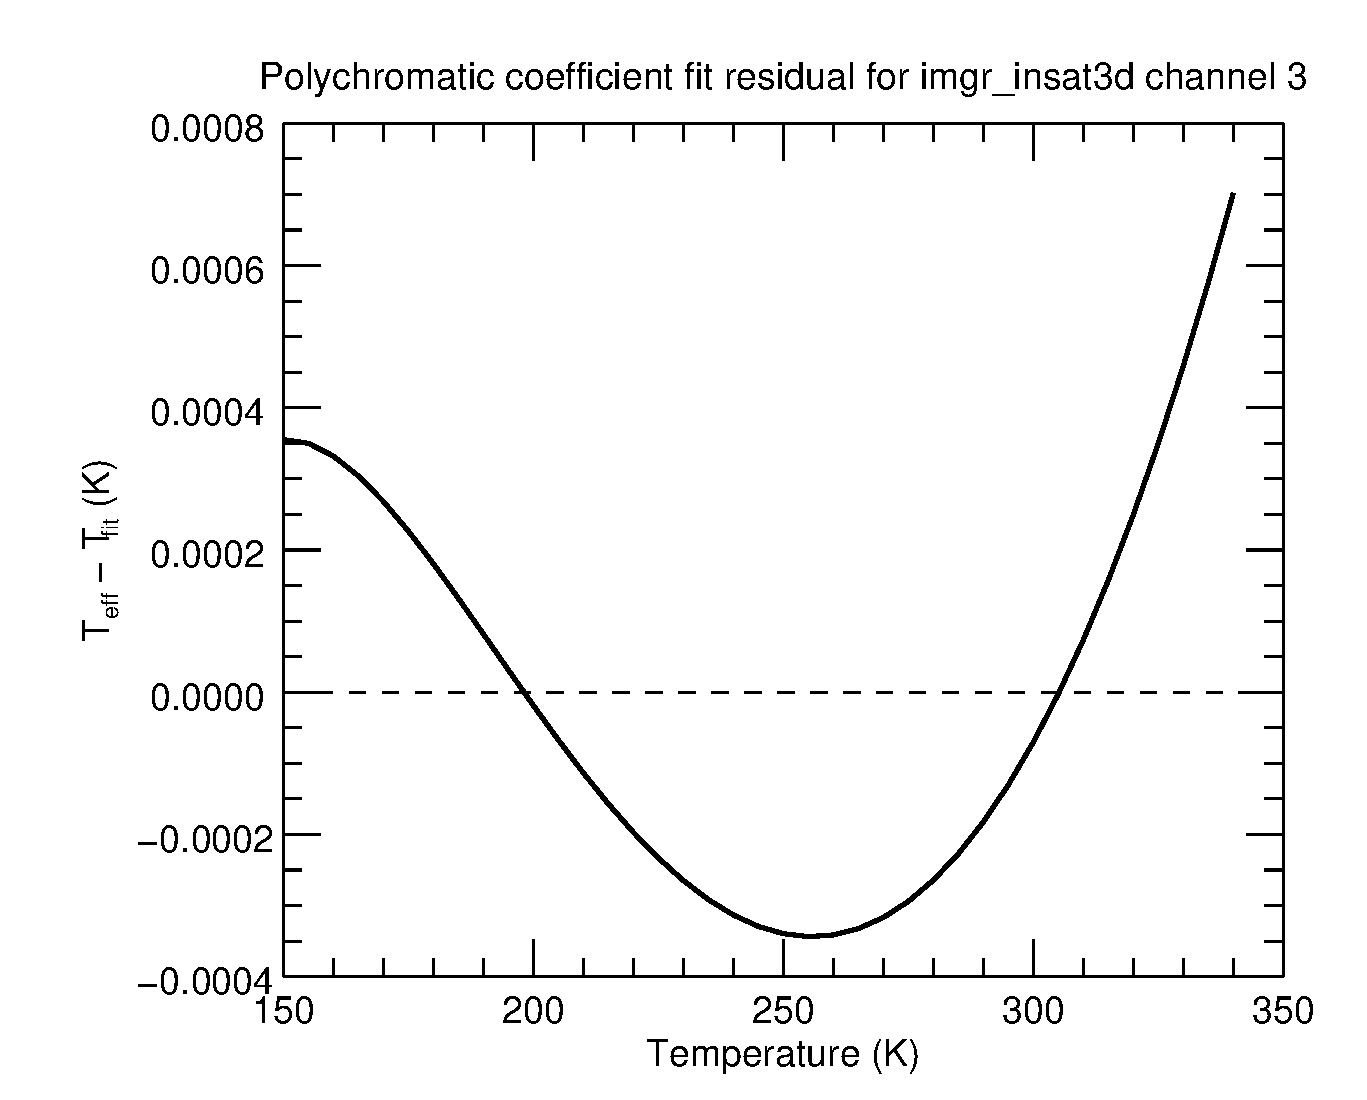
\includegraphics[scale=0.35]{graphics/imgr/tfit/imgr_insat3d-3.tfit.eps} &
    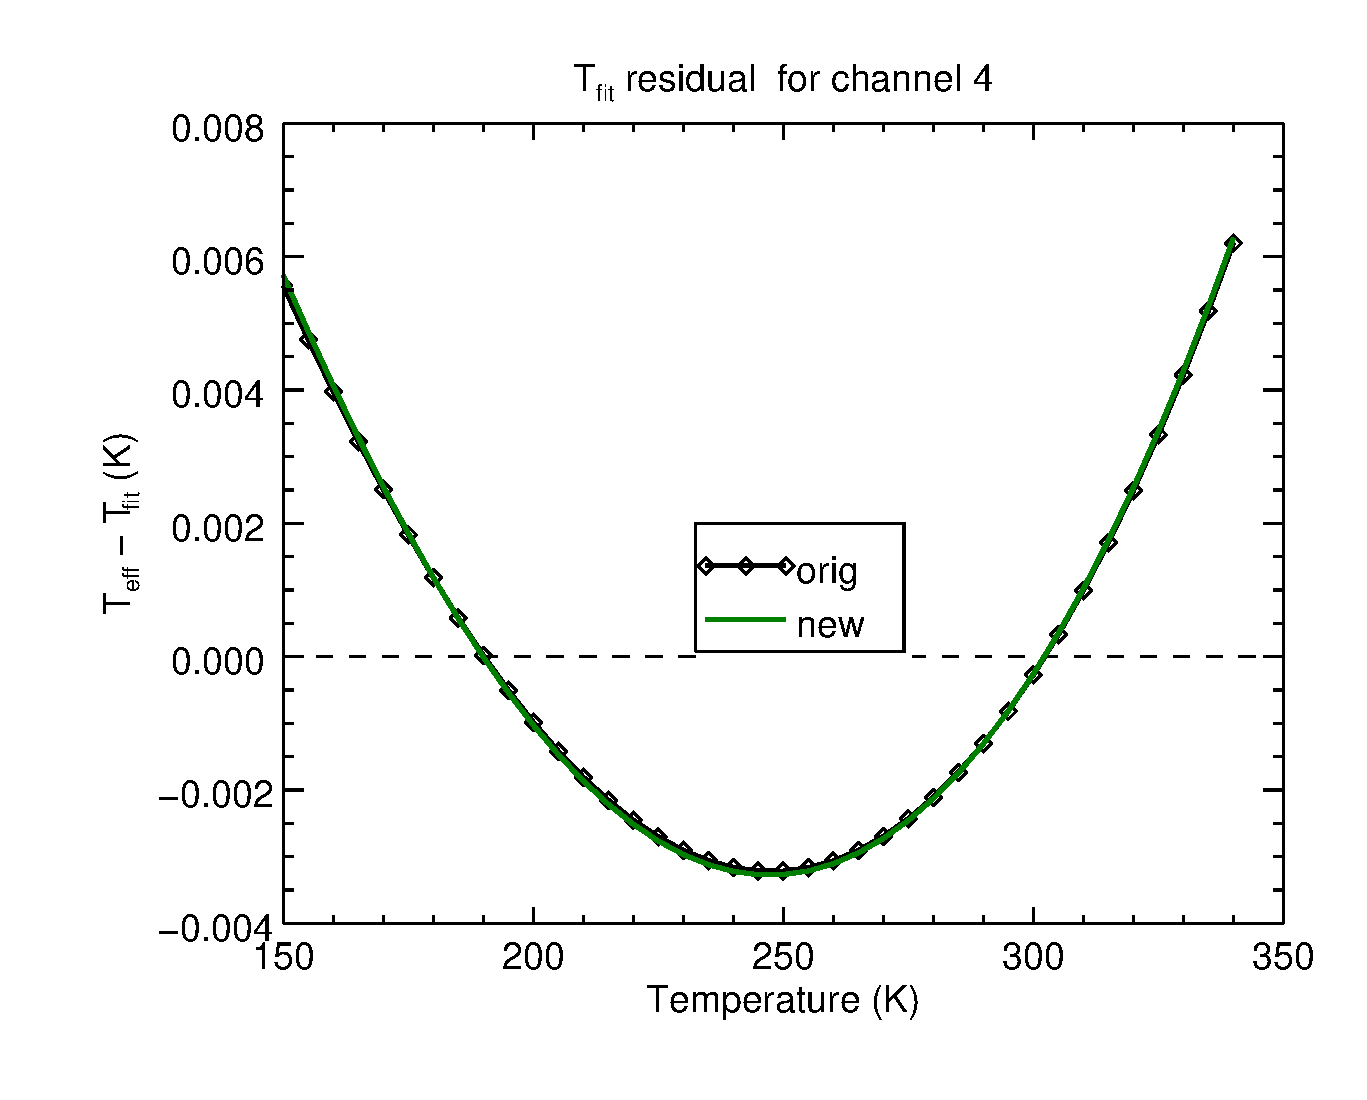
\includegraphics[scale=0.35]{graphics/imgr/tfit/imgr_insat3d-4.tfit.eps} \\\\
    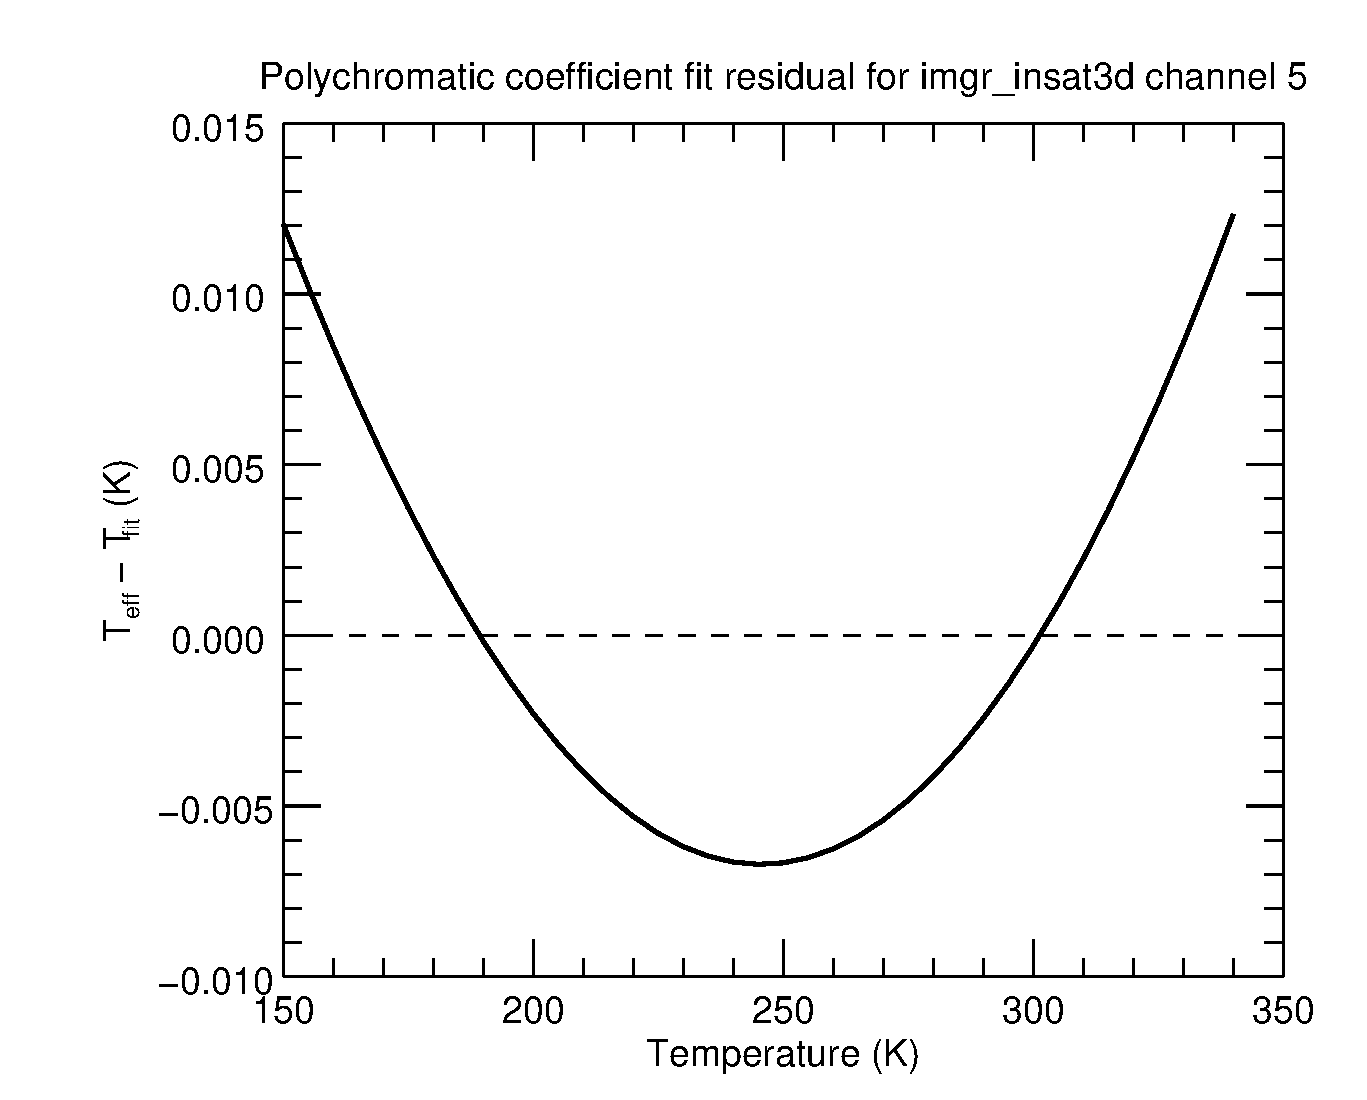
\includegraphics[scale=0.35]{graphics/imgr/tfit/imgr_insat3d-5.tfit.eps} &
    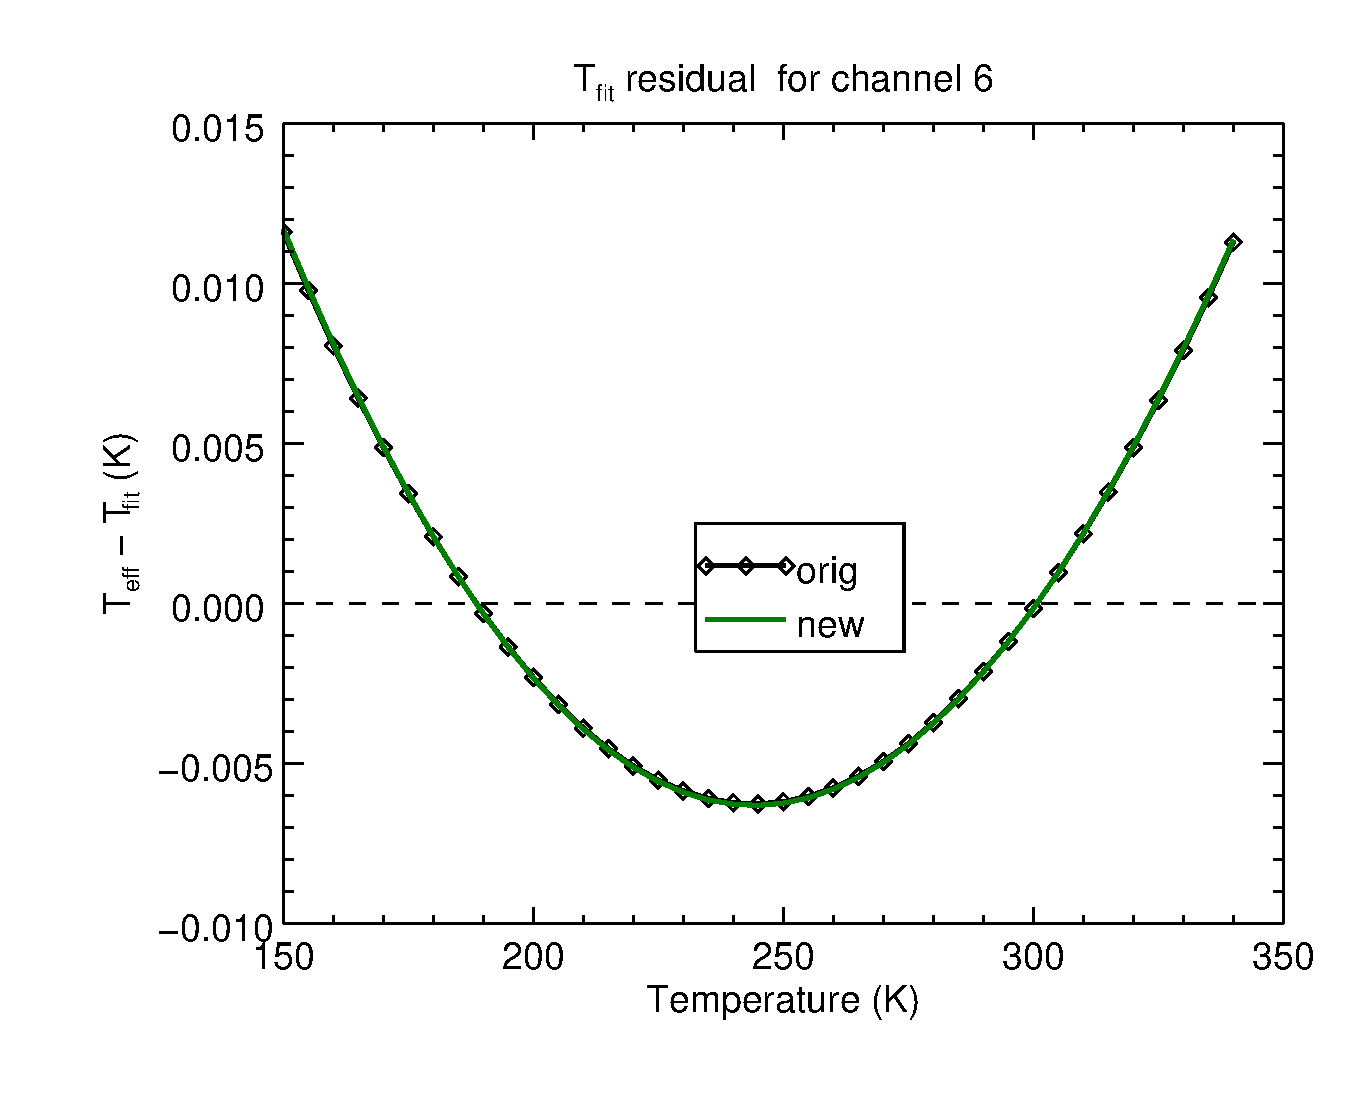
\includegraphics[scale=0.35]{graphics/imgr/tfit/imgr_insat3d-6.tfit.eps} \\
  \end{tabular}
  \caption{INSAT-3D Imager channels 3-6 polychromatic correction temperature fit residuals.}
  \label{fig:imgr_ch1-6_tfit}
\end{figure}

\subsection{Sounder}
%------------------

\addcontentsline{toc}{subsubsection}{Channels 1-6}
\begin{figure}[H]
  \centering
  \begin{tabular}{c c}
    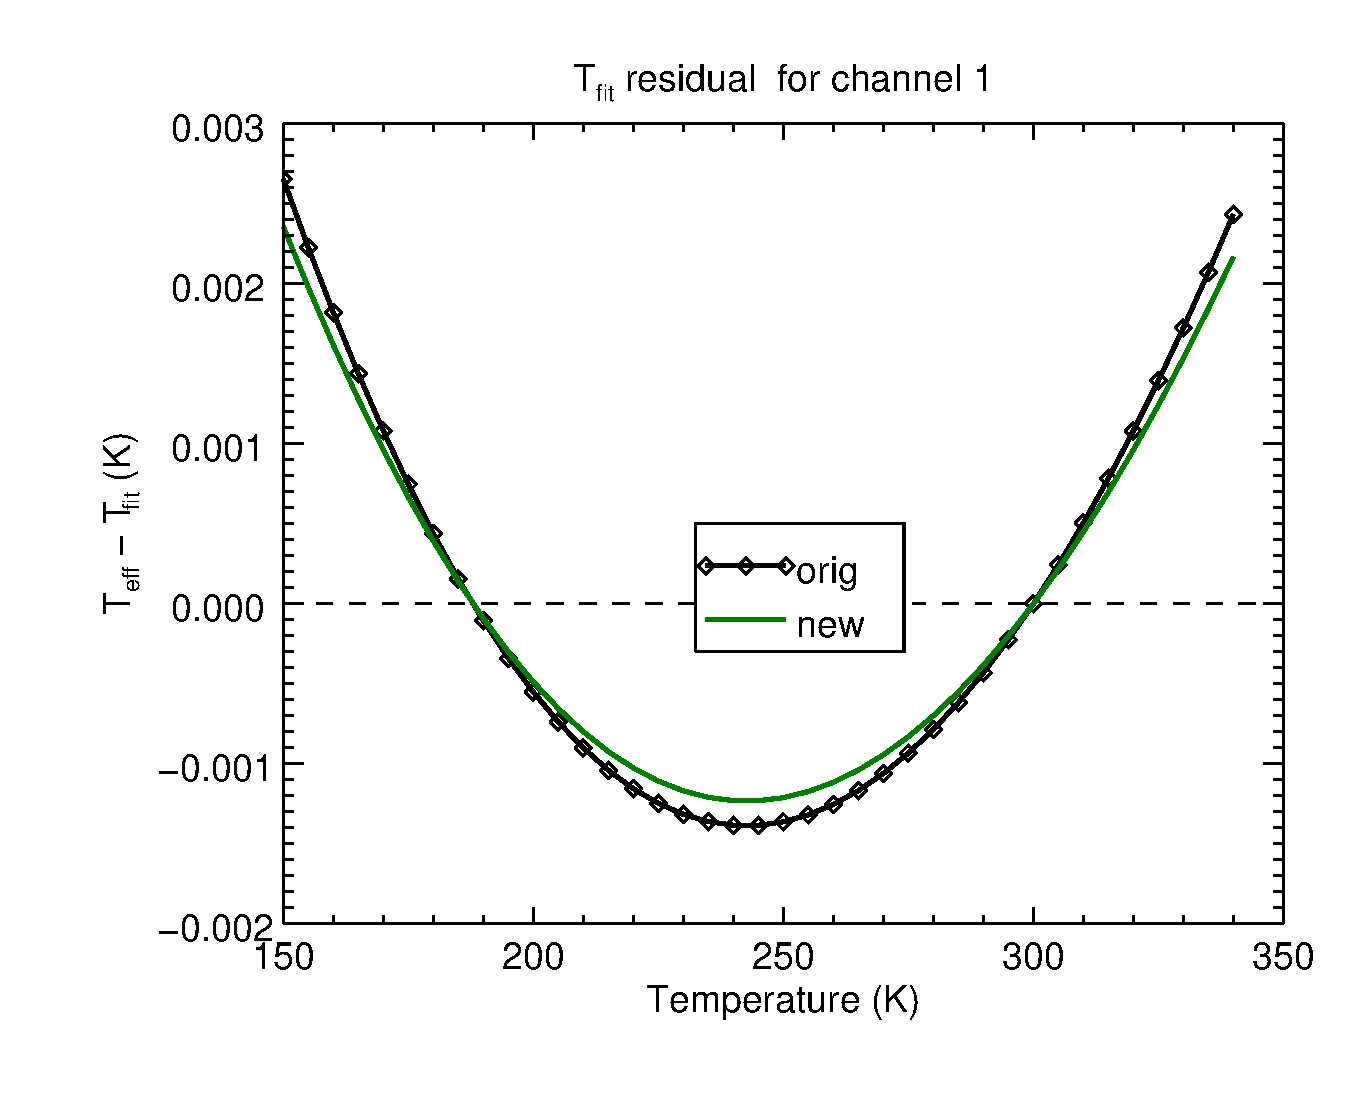
\includegraphics[scale=0.35]{graphics/sndr/tfit/sndr_insat3d-1.tfit.eps} &
    \includegraphics[scale=0.35]{graphics/sndr/tfit/sndr_insat3d-2.tfit.eps} \\\\
    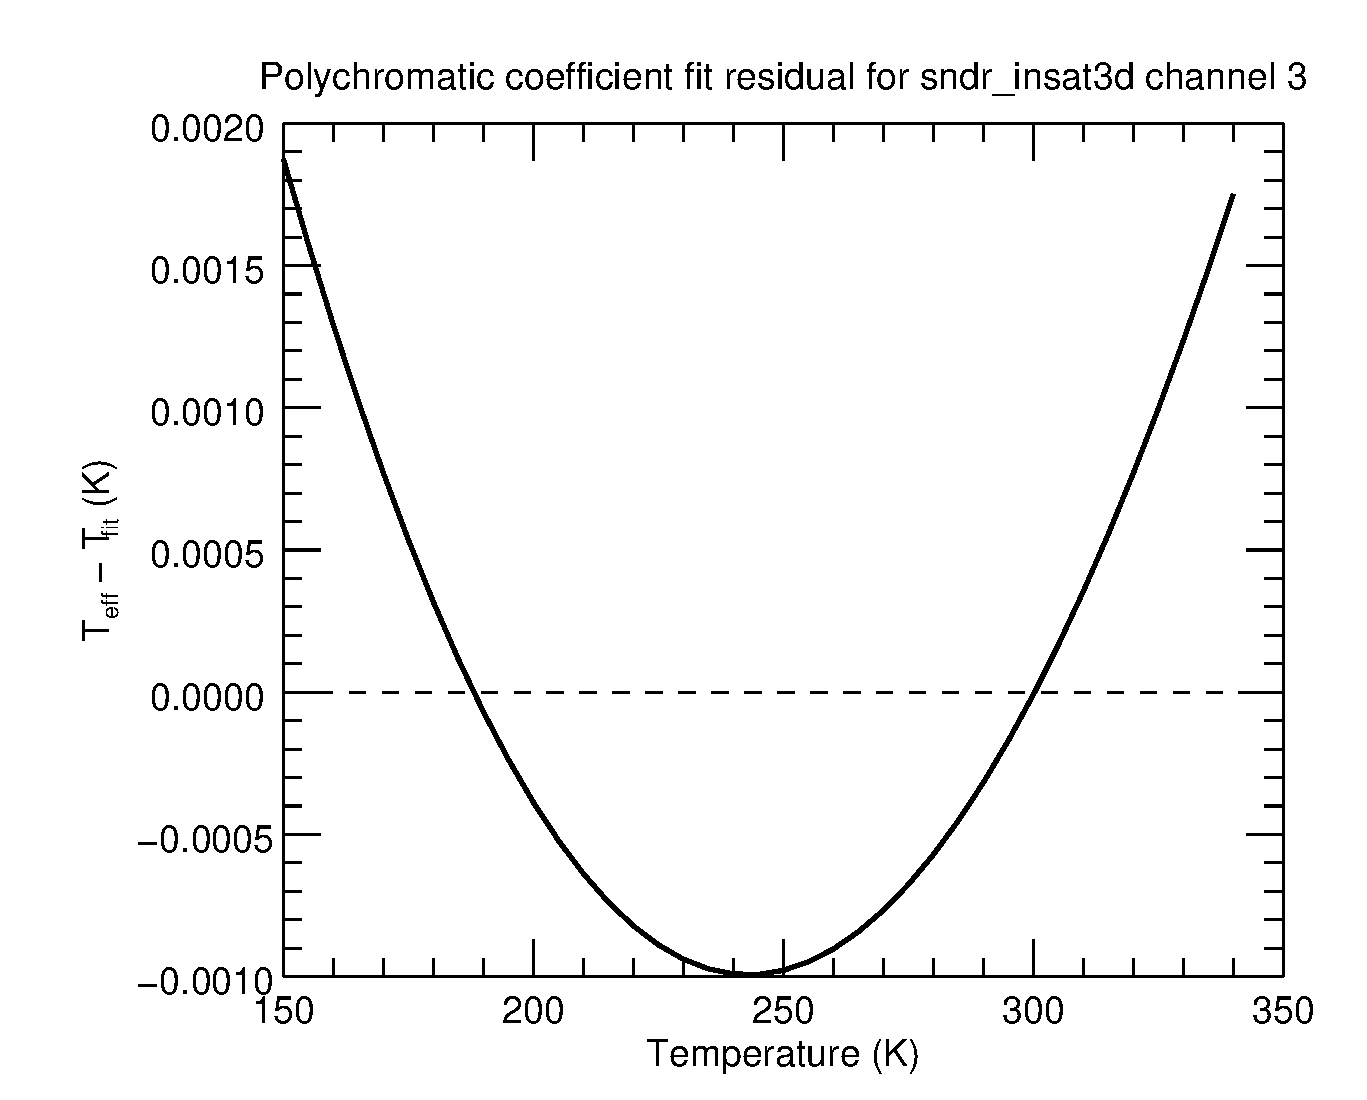
\includegraphics[scale=0.35]{graphics/sndr/tfit/sndr_insat3d-3.tfit.eps} &
    \includegraphics[scale=0.35]{graphics/sndr/tfit/sndr_insat3d-4.tfit.eps} \\\\
    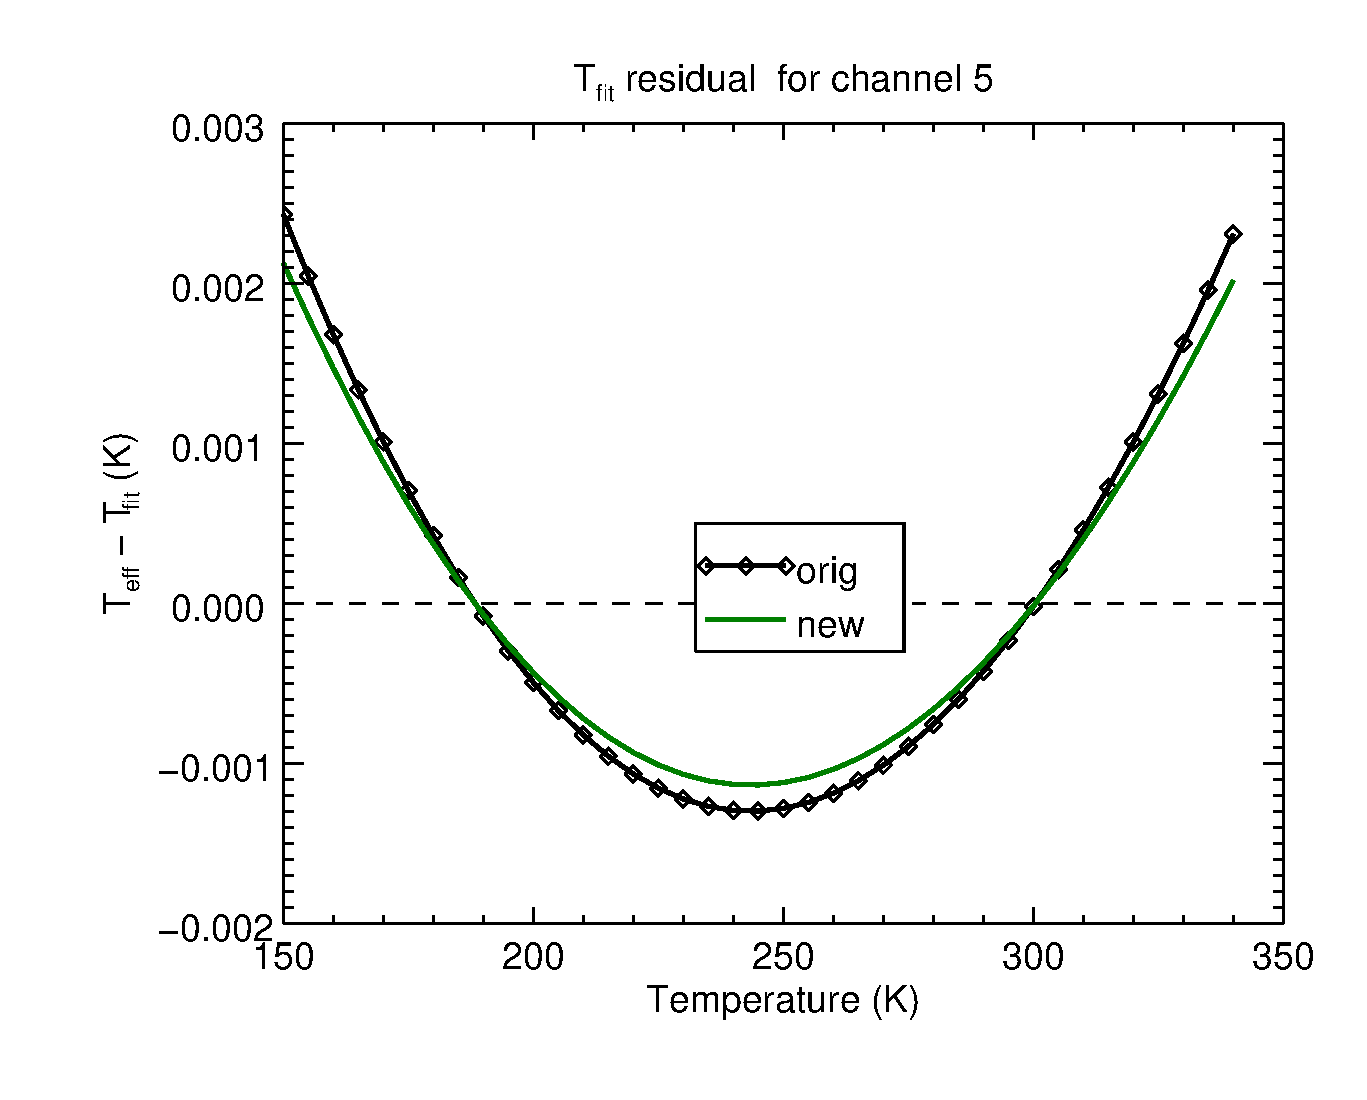
\includegraphics[scale=0.35]{graphics/sndr/tfit/sndr_insat3d-5.tfit.eps} &
    \includegraphics[scale=0.35]{graphics/sndr/tfit/sndr_insat3d-6.tfit.eps} \\
  \end{tabular}
  \caption{INSAT-3D Sounder channels 1-6 polychromatic correction temperature fit residuals.}
  \label{fig:sndr_ch1-6_tfit}
\end{figure}

\addcontentsline{toc}{subsubsection}{Channels 7-12}
\begin{figure}[H]
  \centering
  \begin{tabular}{c c}
    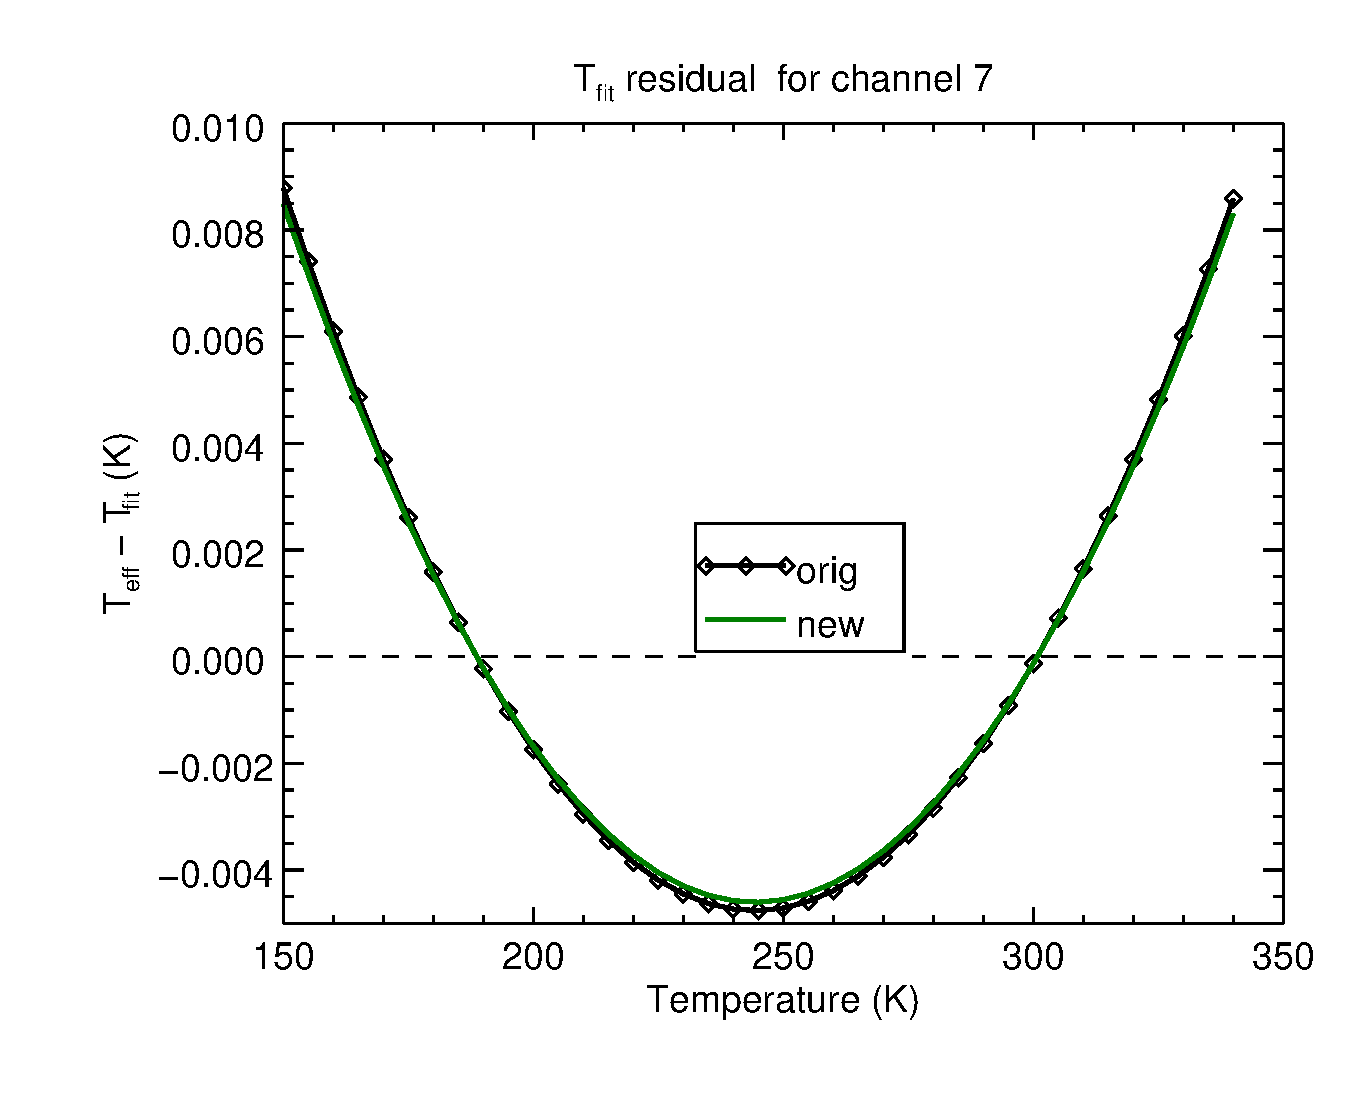
\includegraphics[scale=0.35]{graphics/sndr/tfit/sndr_insat3d-7.tfit.eps} &
    \includegraphics[scale=0.35]{graphics/sndr/tfit/sndr_insat3d-8.tfit.eps} \\\\
    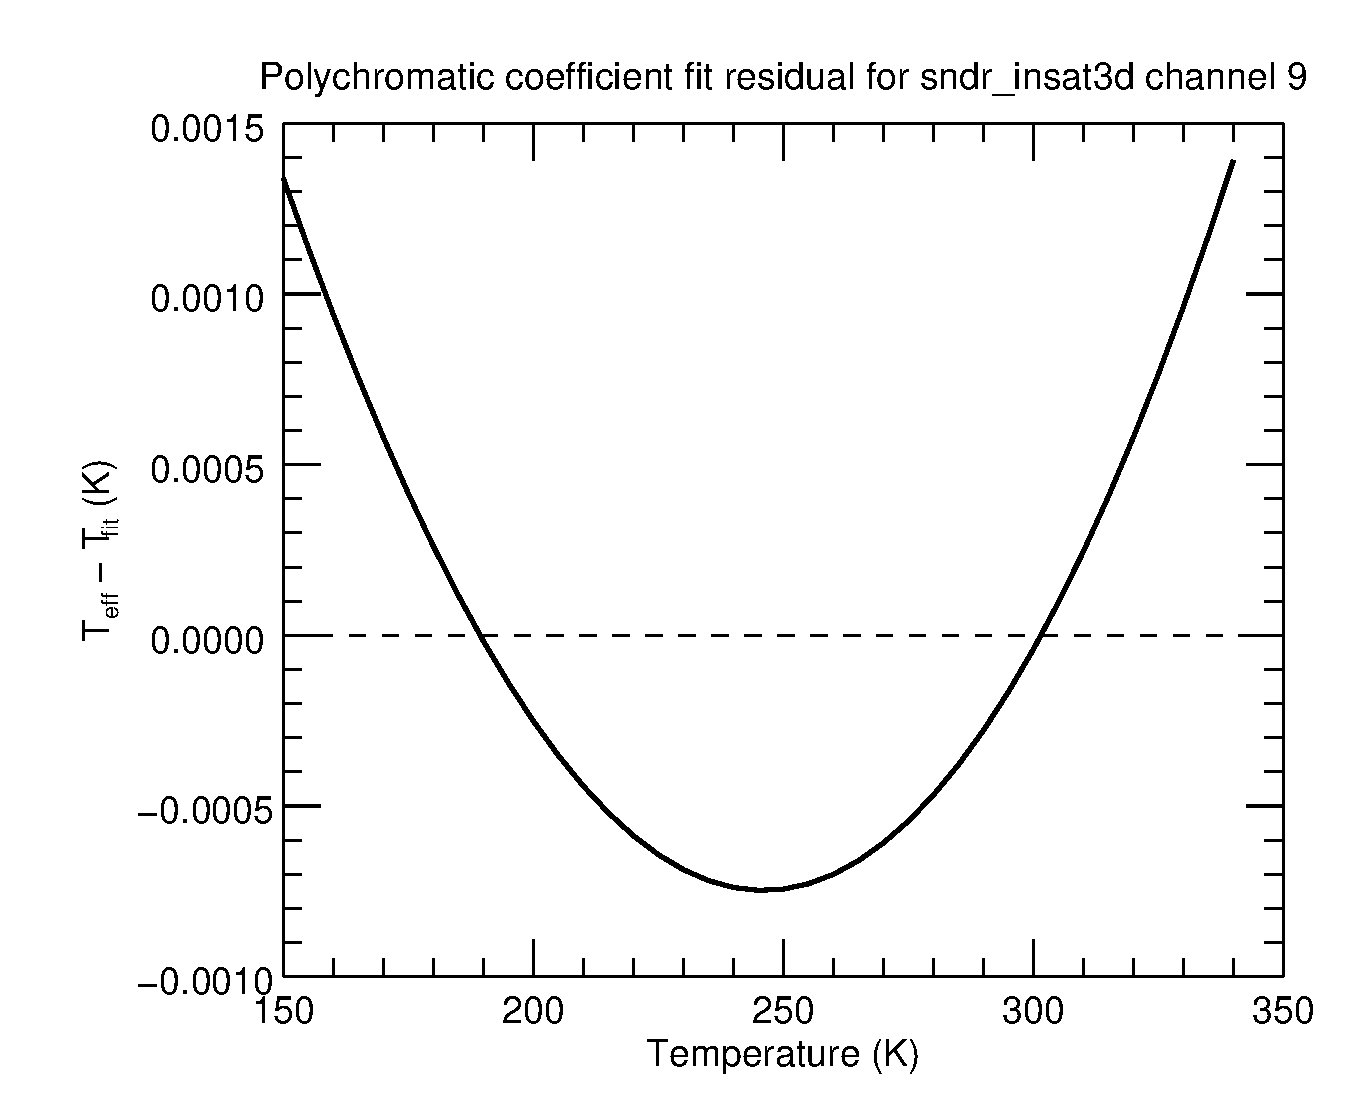
\includegraphics[scale=0.35]{graphics/sndr/tfit/sndr_insat3d-9.tfit.eps} &
    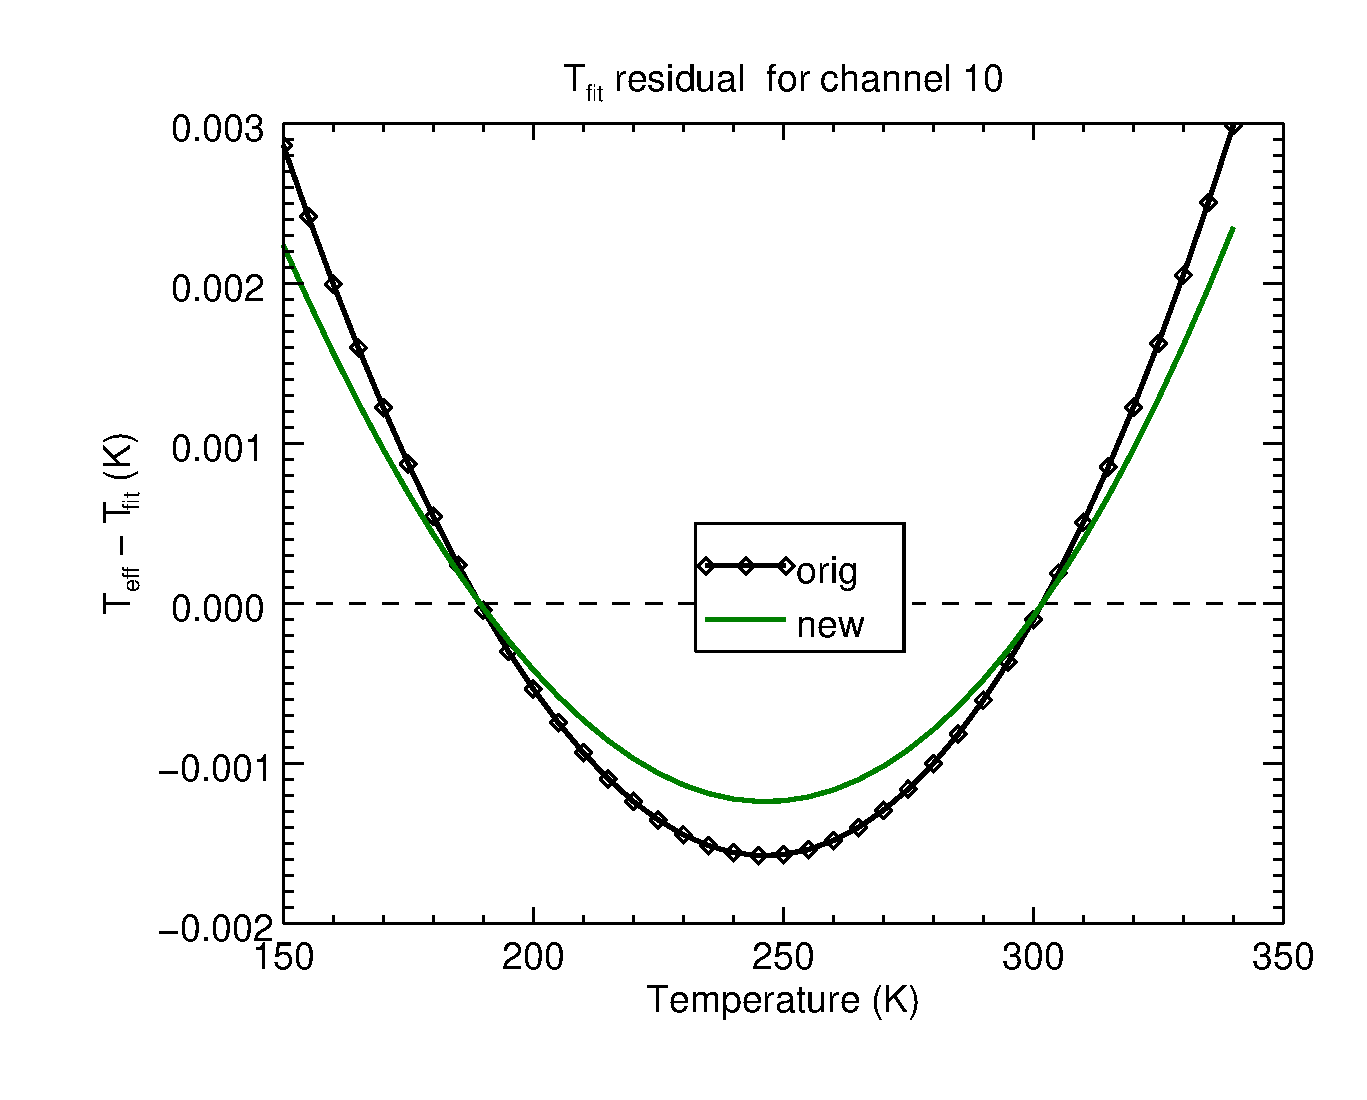
\includegraphics[scale=0.35]{graphics/sndr/tfit/sndr_insat3d-10.tfit.eps} \\\\
    \includegraphics[scale=0.35]{graphics/sndr/tfit/sndr_insat3d-11.tfit.eps} &
    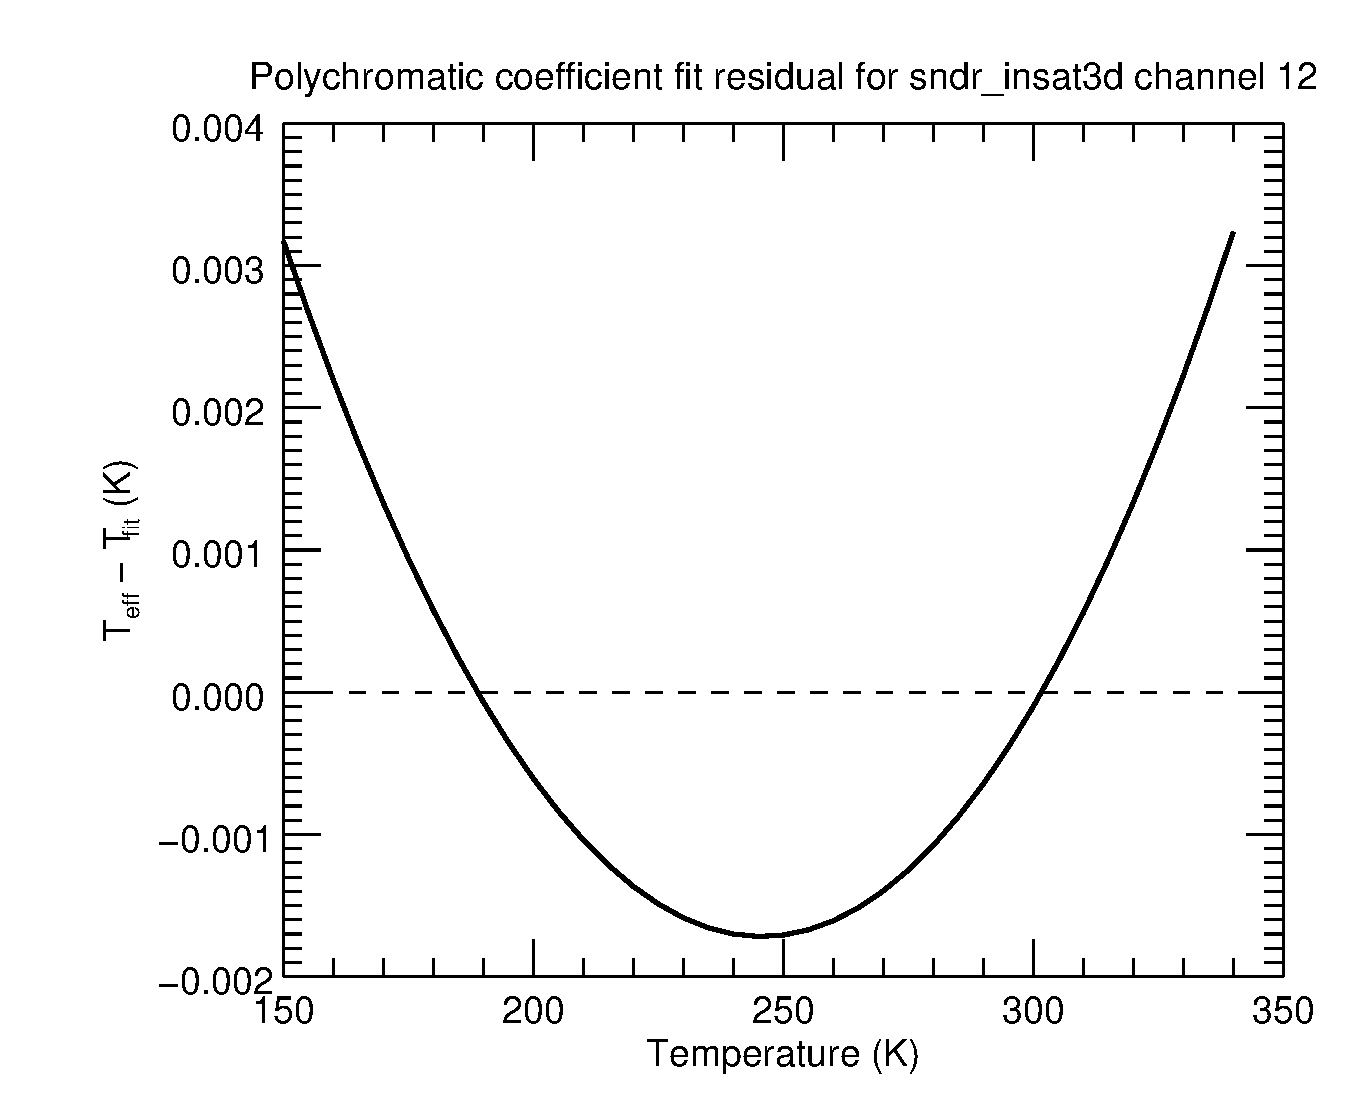
\includegraphics[scale=0.35]{graphics/sndr/tfit/sndr_insat3d-12.tfit.eps} \\
  \end{tabular}
  \caption{INSAT-3D Sounder channels 7-12 polychromatic correction temperature fit residuals.}
  \label{fig:sndr_ch7-12_tfit}
\end{figure}

\addcontentsline{toc}{subsubsection}{Channels 13-18}
\begin{figure}[H]
  \centering
  \begin{tabular}{c c}
    \includegraphics[scale=0.35]{graphics/sndr/tfit/sndr_insat3d-13.tfit.eps} &
    \includegraphics[scale=0.35]{graphics/sndr/tfit/sndr_insat3d-14.tfit.eps} \\\\
    \includegraphics[scale=0.35]{graphics/sndr/tfit/sndr_insat3d-15.tfit.eps} &
    \includegraphics[scale=0.35]{graphics/sndr/tfit/sndr_insat3d-16.tfit.eps} \\\\
    \includegraphics[scale=0.35]{graphics/sndr/tfit/sndr_insat3d-17.tfit.eps} &
    \includegraphics[scale=0.35]{graphics/sndr/tfit/sndr_insat3d-18.tfit.eps} \\
  \end{tabular}
  \caption{INSAT-3D Sounder channels 13-18 polychromatic correction temperature fit residuals.}
  \label{fig:sndr_ch13-18_tfit}
\end{figure}

\end{appendix}

\end{document}

